\documentclass[conference]{IEEEtran}
\usepackage{amsmath,amssymb}
\usepackage{graphicx}
\usepackage{cite}
\usepackage{booktabs}
\usepackage{tikz}
\usetikzlibrary{arrows.meta,positioning,fit,backgrounds,calc}
\usepackage{url}
\usepackage{xcolor}
\IEEEoverridecommandlockouts

% ---------------------------------------------------------------------------
% NOTATION (not printed): plain Latin letters with stated meanings.
% See the Notation paragraph at the start of Sec. III.
% ---------------------------------------------------------------------------

% ---------------------------------------------------------------------------
% Figure placeholder helper: if the graphic exists it is included; otherwise a
% labelled placeholder box is drawn so the document always compiles.
% Remove this macro (and use \includegraphics directly) once all figures exist.
% ---------------------------------------------------------------------------
\newcommand{\figph}[3]{%
  \IfFileExists{#1}%
    {\includegraphics[width=#2]{#1}}%
    {\setlength{\fboxsep}{0pt}%
     \fbox{\begin{minipage}[c][#3][c]{\dimexpr#2-2\fboxrule\relax}%
       \centering\footnotesize\color{red!70!black}%
       [FIGURE PLACEHOLDER]\\[2pt]
       {\ttfamily\scriptsize\detokenize{#1}}%
     \end{minipage}}}%
}

\begin{document}

\title{Real-Time Cardiac Field Artifact Removal in Ear-EEG\\Using Heart-Beat Timing-Based Iterative Learning Control}

\author{
Wenlin Zhang$^{1}$, Sam Lin$^{1,6}$, Shuai Li$^{3}$, Ye Yuan$^{1}$,\\
Zheng Wang$^{1,2}$, Tony Ni$^{4}$, Kant Yao$^{4}$, Yongcheng Li$^{5}$, Davide Momi$^{7}$%
\thanks{\footnotesize
$^{1}$Institute of Brain and Mind, CA, USA\protect\\
$^{2}$Krembil Centre for Neuroinformatics, Centre for Addiction and Mental Health, Toronto, Ontario, Canada\protect\\
$^{3}$University of Oulu, Oulu, Finland\protect\\
$^{4}$Synchroni Scientific Instruments Inc., Canada\protect\\
$^{5}$Shenzhen Institutes of Advanced Technology, China\protect\\
$^{6}$Palos Verdes Peninsula High School, CA, USA\protect\\
$^{7}$University of California, Irvine, CA, USA\protect\\
\textit{Corresponding author: [Name] (e-mail: [corresponding.author@institute.edu]).}
}
}

\maketitle

\begin{abstract}
Continuous wearable EEG is increasingly co-worn with consumer devices that already stream a
heartbeat signal, creating a practical opportunity for reference-driven cardiac artifact removal in
low-channel ear-EEG where blind source separation is channel-starved. We report a measurement that
reshapes how that opportunity should be used. On a real behind-the-ear EEG and chest-ECG recording
(SeizeIT2/ds005873, 10~min, 717 beats), magnitude-squared coherence between the ECG reference and
the ear-EEG channel is near zero---$6\times10^{-10}$ over 8--20~Hz whole-record, and only
$0.11$ on average even under best-case R-locked beat-synchronous pooling. The cardiac field artifact
reaching the ear is therefore \emph{phase-locked but waveform-decorrelated} from the ECG lead, which
rules out reference-driven waveform regression (LMS/RLS and Hammerstein-style residual cancellers)
and motivates a \emph{timing-only} design. Yet R-anchored synchronous averaging on the same
recording recovers a clear, repeatable per-beat template, confirming the artifact is genuinely
timing-repeatable. We exploit exactly this structure with a two-level (min/max) envelope tracker and
PI phase-locked tracker that produce robust beat timing and continuous cardiac phase under amplitude
drift, followed by phase-anchored iterative learning control (ILC) that learns and subtracts the
repeatable template. Because only beat \emph{timing} is required, a cross-device heartbeat source
(e.g., a smartwatch) is sufficient. We analyze non-causal, buffered-causal (one-beat latency), and
strict-causal (zero-latency) modes on real data: buffered matches the non-causal upper bound
(R-spike $50.2$ vs.\ $50.7\,\mu$V) while strict-causal is capped by RR-prediction error
($34.7\,\mu$V, $-32\%$). The online path costs $O(1)$ per sample with $O(L_w)$ memory, suitable for
always-on wearable execution.
\end{abstract}

\begin{IEEEkeywords}
Ear-EEG, cardiac field artifact, iterative learning control, repetitive control, phase-locked loop,
coherence analysis, smartwatch, real-time, wearable.
\end{IEEEkeywords}

% ===========================================================================
\section{Introduction}

\textbf{Vision.} Wearable EEG is moving toward continuous, day-scale monitoring in earable form
factors, and a large fraction of prospective users already wear a second device---a smartwatch or
band---that exposes a heartbeat stream from ECG or PPG. This suggests a practical multimodal path:
use the heartbeat signal that is \emph{already available} to stabilize artifact removal in a
low-channel ear-EEG device, without adding electrodes, wiring, or setup burden to the headset
itself. The question this paper answers is what form that assistance can actually take.

\textbf{Why cardiac artifact, and why at the ear.} The cardiac field artifact (CFA) is the
volume-conducted electrical potential of the heart's dipole appearing at recording
electrodes~\cite{dirlich1997}. It is distinct from the ballistocardiogram (BCG) motion artifact
studied in simultaneous EEG-fMRI~\cite{allen1998,allen2000,niazy2005}; for out-of-scanner earables
CFA is the relevant cardiac contamination. Its relative severity grows in ear-centered montages,
where electrodes sit near the neck and large-vessel pathways while the neural signal of interest is
comparatively small.

\textbf{The constraint stack.} Four deployment constraints jointly determine which methods are
admissible, and it is their conjunction that is restrictive. \textbf{(C1)}~\emph{Channel
starvation}: earables provide few channels ($C<8$), placing blind source separation at or beyond its
identifiability limit~\cite{jung2000,pion2019}. \textbf{(C2)}~\emph{Always-on power}: a
coin-cell-class budget excludes deep denoisers and heavy per-sample linear algebra.
\textbf{(C3)}~\emph{Causality}: interactive use requires real-time output.
\textbf{(C4)}~\emph{Reference modality}: a cross-device heartbeat source supplies reliable beat
\emph{timing}, but not a sample-aligned \emph{waveform}---independent clocks and wireless transport
introduce unknown, drifting latency.

\textbf{The measurement that settles the design.} Constraint (C4) raises an empirical question: even
with a co-recorded, wired ECG lead, is the ear-EEG artifact waveform predictable from the reference
waveform at all? We find it is not---coherence is indistinguishable from zero whole-record and
remains near $0.11$ even when every timing advantage is granted through R-locked beat-synchronous
pooling (\S\ref{sec:coh}). Reference-driven \emph{waveform} regression therefore has essentially
nothing to regress against, independent of (C1)--(C3). What survives is \emph{timing}: the same
recording yields a clear, repeatable R-anchored template (\S\ref{sec:template}). The design that
follows is timing-only by necessity---and timing is exactly what a cross-device source can deliver.

\textbf{Contributions.} \textbf{C1)} An empirical coherence analysis on real ear-EEG/ECG showing the
cardiac artifact at the ear is phase-locked but waveform-decorrelated, ruling out reference-driven
residual cancellers in this configuration. \textbf{C2)} A timing-only synthesis: a min/max envelope
tracker with PI phase tracking and arrhythmia-aware supervision feeding a phase-anchored ILC
canceller. \textbf{C3)} A real-data analysis of non-causal, buffered-causal, and strict-causal
operation, quantifying the latency-versus-suppression tradeoff set by RR predictability.
\textbf{C4)} A constant-time complexity profile and comparison against reference-driven and BSS
baselines under ground-truth-free metrics.

% ===========================================================================
\section{Related Work}

LMS/NLMS/RLS cancellation with an ECG reference is
textbook~\cite{widrow1975,haykin2014,sayed2008,diniz2013}; residuals arise from channel-specific
volume conduction, QRS morphology mismatch, and nonstationarity. All such methods presuppose the
artifact is predictable from the reference waveform---the assumption we test in \S\ref{sec:coh}.
Average artifact subtraction and optimal-basis-set refinement were developed for the BCG artifact in
EEG-fMRI~\cite{allen1998,allen2000,niazy2005}; once epochs are QRS-aligned that repeatable-template
machinery ports to CFA, and we adopt it inside a control framework. ICA~\cite{jung2000} with
automated labeling~\cite{pion2019} and artifact subspace reconstruction~\cite{mullen2015} are
standard for multichannel wearable EEG but are limited by (C1). Deep denoisers and benchmarks
(e.g.,~\cite{zhang2021}) chiefly target ocular and muscular artifacts and are costly under (C2);
algorithm unrolling~\cite{gregor2010,monga2021} is a possible low-power route compatible with this
design. Rejection of periodic exogenous disturbances is the province of repetitive control, grounded
in the internal model principle~\cite{francis1976,hara1988,longman2000}, and of ILC for repeating
trials~\cite{arimoto1984,bristow2006}---mature and production-proven in mechatronics but essentially
absent from EEG artifact removal. Reframing CFA as heartbeat-timed periodic-disturbance rejection is
the central move here; the synchronous-averaging step is the direct analogue of repeatable-runout
separation in disk servo control, where the repeatable component is extracted from an index pulse
alone, never a waveform reference.

% ===========================================================================
\section{Signal Model and Design Rationale}

\textbf{Notation.} All quantities use plain Latin letters. Signals: $y(t)$ measured ear-EEG channel;
$s(t)$ neural signal of interest; $d(t)$ cardiac disturbance; $n(t)$ channel noise; $r(t)$ heartbeat
reference (ECG or PPG). Timing: $t_k$ the $k$-th R-peak instant; $\mathrm{RR}_k=t_{k+1}-t_k$;
$p(t)\in[0,1)$ the cardiac phase; $o(t)$ the time-since-R offset. Method: $m(o)$ the ILC template;
$L_w$ its length; $a$ the ILC learning gain; $q$ the $Q$-filter/forgetting factor; $pk(t),bl(t)$ the
peak and baseline trackers; $g(t)$ the normalized gate; $l[k]$ the per-beat learn-gate.

The measured channel is
\begin{equation}
y(t) = s(t) + d(t) + n(t).
\label{eq:meas}
\end{equation}
Systole (QRST) is approximately time-locked to the R-peak while diastole absorbs most of the RR
variation, so we anchor a repeatable component in time-since-R and treat the remainder as drift,
\begin{equation}
d(t) = d_p\big(t - t_k\big) + d_r(t),
\label{eq:decomp}
\end{equation}
where $d_p$ is the beat-repeatable component and $d_r$ collects beat-to-beat variation driven by
heart-rate variability, respiration, and posture.

\textbf{Design rationale.} Two properties of $d(t)$ can be exploited, and they are independent:
predictability from the reference \emph{waveform} (measured by coherence) and repeatability across
beats given only the reference \emph{timing} (exploited by synchronous averaging). Our measurement
(\S\ref{sec:coh}) finds the former absent and the latter present, so the method targets $d_p$ using
$t_k$ alone. Consequently $d_r$ is \emph{not} addressable by a reference-driven residual stage here,
and we do not claim it---a scope restriction imposed by the data. Since the reference enters only
through $t_k$, a non-sample-aligned heartbeat source suffices: the cross-device latency of (C4)
shifts $t_k$ by a slowly-varying offset, which the phase-locked tracker absorbs.

% ===========================================================================
\section{Proposed Method}

Fig.~\ref{fig:sys} shows the signal flow: the heartbeat reference $r(t)$ drives a phase estimator
whose outputs $(t_k,p(t),l[k])$ anchor and gate an ILC template canceller acting on $y(t)$.

\begin{figure}[t]
\centering
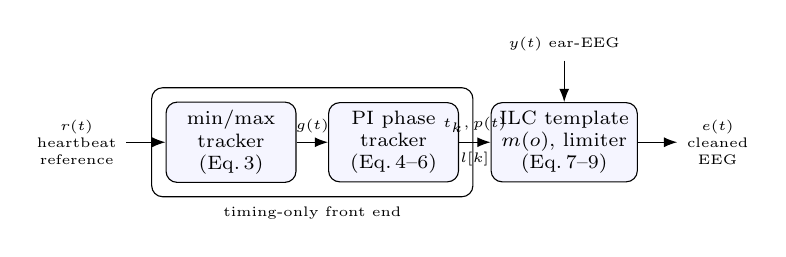
\begin{tikzpicture}[
  font=\scriptsize,
  blk/.style={draw, rectangle, rounded corners, minimum height=0.85cm, align=center, inner sep=3pt, fill=blue!4},
  lbl/.style={font=\tiny, align=center},
  >=Latex, node distance=4mm
]
\node[lbl] (r) at (0,0) {$r(t)$\\heartbeat\\reference};
\node[blk, minimum width=1.65cm, right=5mm of r] (trk) {min/max\\tracker\\(Eq.\,3)};
\node[blk, minimum width=1.65cm, right=4mm of trk] (pll) {PI phase\\tracker\\(Eq.\,4--6)};
\node[blk, minimum width=1.7cm, right=4mm of pll] (ilc) {ILC template\\$m(o)$, limiter\\(Eq.\,7--9)};
\node[lbl, right=5mm of ilc] (e) {$e(t)$\\cleaned\\EEG};
\node[lbl] (y) at ($(ilc)+(0,1.25)$) {$y(t)$ ear-EEG};

\draw[->] (r) -- (trk);
\draw[->] (trk) -- node[above,lbl]{$g(t)$} (pll);
\draw[->] (pll) -- node[above,lbl]{$t_k,p(t)$}node[below,lbl]{$l[k]$} (ilc);
\draw[->] (y) -- (ilc);
\draw[->] (ilc) -- (e);
\begin{pgfonlayer}{background}
\node[draw, rounded corners, fit=(trk)(pll), inner sep=5pt,
      label={[lbl]below:timing-only front end}] {};
\end{pgfonlayer}
\end{tikzpicture}
\caption{Signal flow. Only beat \emph{timing} crosses from the reference to the canceller; the ECG
waveform is never used as a regressor, which is what permits a cross-device heartbeat source.}
\label{fig:sys}
\end{figure}

\subsection{Phase estimator: min/max tracker with PI phase tracking}
A QRS-emphasis band-pass feeds two streaming trackers: a peak tracker $pk(t)$ (fast attack, slow
release) and a baseline tracker $bl(t)$ (slow moving average). The normalized gate
\begin{equation}
g(t) = \frac{r(t) - bl(t)}{pk(t) - bl(t)}
\label{eq:gate}
\end{equation}
is amplitude-drift invariant, so posture and contact-impedance drift do not defeat detection---a
fixed threshold would. Schmitt hysteresis plus a 250~ms refractory yield clean beat gating; the
fiducial $t_k$ is the raw-reference maximum inside the gated window, which minimizes jitter relative
to using the band-passed envelope.

A PI phase-locked tracker converts sparse fiducials into a continuous phase. Between beats the phase
free-runs at the current rate estimate,
\begin{equation}
p(t+1) = \big[\,p(t) + \mathrm{fr}(t)\,\big] \bmod 1, \quad
\mathrm{fr}(t) = \frac{1}{\mathrm{RR}_{\mathrm{est}}(t)\,f_s},
\label{eq:phaseacc}
\end{equation}
with $f_s$ the sample rate. At each fiducial a proportional term realigns phase and an integral term
tracks the rate,
\begin{align}
p &\leftarrow p - K_p\,e_p, \label{eq:pcorr}\\
\mathrm{RR}_{\mathrm{est}} &\leftarrow \mathrm{RR}_{\mathrm{est}}
  + K_i\,\big(\mathrm{RR}_{\mathrm{meas}} - \mathrm{RR}_{\mathrm{est}}\big),
\label{eq:rcorr}
\end{align}
where $e_p$ is the wrapped phase error. The loop bandwidth is set above respiratory sinus arrhythmia
(RSA, $\sim$0.2--0.4~Hz) so the tracker follows breathing-driven rate modulation, and below per-beat
detection noise so isolated fiducial errors are averaged out. Free-running \eqref{eq:phaseacc} also
\emph{predicts} the next R-instant, which is what enables the strict-causal mode below.

An arrhythmia supervisor classifies each beat by
$\mathrm{RR}_{\mathrm{meas}}/\mathrm{RR}_{\mathrm{est}}$ and applies the matching reflex.
\emph{Premature}: trust the measured phase (the beat did occur), but freeze the rate integrator and
set $l[k]=0$. \emph{Missed}: trust the prediction, retain the rate, and set $l[k]=0$. This prevents
a single anomalous beat from corrupting either the rate state or the learned template.

\subsection{Phase-anchored ILC template cancellation}
A template $m(o)$ indexed by time-since-R offset stores $d_p$. Cancellation is a table lookup,
\begin{equation}
e(t) = y(t) - \mathrm{sat}_{\pm\beta\,pk(t)}\big(m(o(t))\big),\quad \beta\in(0,1),
\label{eq:cancel}
\end{equation}
where $\mathrm{sat}_{\pm L}(x)=\max(-L,\min(L,x))$ caps the subtracted amount at a fraction $\beta$
of the tracked reference amplitude, bounding worst-case over-subtraction. Learning is a first-order
ILC (leaky-integrator) update applied only on supervisor-approved beats ($l[k]=1$),
\begin{equation}
m(o) \leftarrow q\,m(o) + a\,e(t).
\label{eq:learn}
\end{equation}
Because we estimate an \emph{additive disturbance} rather than invert a plant, the effective plant is
the identity and the ILC convergence condition reduces to $|q(1-a)|<1$, satisfied for any
$a\in(0,1]$, $q\in(0,1]$. The factor $q$ trades asymptotic cancellation depth against drift tracking.

\emph{Why this does not remove neural signal.} \eqref{eq:learn} is structurally an evoked average,
accumulating only energy consistent across beats at the same offset $o$. Neural activity not
phase-locked to the R-peak averages toward zero in $m(o)$ regardless of frequency, so spectral
overlap between $s(t)$ and $d(t)$ is not by itself a hazard; cancellation is further confined to
$o(t)\in[0,L_w)$. The genuine residual risk is the heartbeat-evoked potential (HEP), which \emph{is}
phase-locked~\cite{park2019}; \eqref{eq:cancel} bounds but does not eliminate this, and we report
alpha preservation as an indirect check (\S\ref{sec:preserve}).

\subsection{Operating modes}
R-peak confirmation lags the true R-instant by $\sim$60--80~ms, which forces a mode choice.
\emph{Non-causal} uses all beats and serves as an offline upper bound. \emph{Buffered-causal}
delays output by approximately one beat so every sample is anchored to its \emph{detected} $t_k$,
recovering the sharp R-spike fully. \emph{Strict-causal} adds no latency and must anchor to the
\emph{predicted} R-instant from \eqref{eq:phaseacc}; the achievable R-spike depth is then capped by
RR-prediction error, which is dominated by RSA-tracking lag. Broad P and T components survive
prediction; only the sharp R deflection is latency-critical. \S\ref{sec:modes} quantifies this on
real data.

\subsection{Complexity}
Tracker updates and gating are constant-time; the PI phase update is constant-time (amortized
per sample); ILC lookup and update are constant-time with memory $L_w$. The proposed online path is
therefore $O(1)$ per sample with $O(L_w)$ memory per channel (Table~\ref{tab:complexity}), with no
matrix operations and no growing state---the profile required by (C2). Reference-driven adaptive
baselines are reported separately and are not part of the deployment path.

\begin{table}[t]
\centering
\caption{Per-sample cost per channel (proposed online path).}
\label{tab:complexity}
\begin{tabular}{@{}lcc@{}}
\toprule
Stage & Time & Memory \\
\midrule
Trackers, gate, supervisor \eqref{eq:gate}            & $O(1)$ & $O(1)$ \\
PI phase tracker \eqref{eq:phaseacc}--\eqref{eq:rcorr} & $O(1)$ & $O(1)$ \\
ILC subtract + learn \eqref{eq:cancel},\eqref{eq:learn} & $O(1)$ & $L_w$ \\
\midrule
\textbf{Total}                                         & $\mathbf{O(1)}$ & $\mathbf{O(L_w)}$ \\
\bottomrule
\end{tabular}
\end{table}

% ===========================================================================
\section{Experimental Analysis}

\subsection{Dataset and protocol}
We analyze a 10-minute segment (717 beats; 2 premature, 0 missed per the supervisor) from
SeizeIT2~\cite{seizeit2} (OpenNeuro ds005873), pairing a wearable behind-the-ear EEG channel at
256~Hz with a synchronized chest ECG lead. This is favorable to reference-driven methods---the ECG
is clean, wired, and genuinely synchronized---so it is a conservative test of the coherence
assumption. Lacking ground-truth $s(t)$, we use ground-truth-free metrics: coherence to the
reference, recovered R-locked template amplitude, cardiac-band power reduction, and alpha
preservation.

\subsection{Coherence analysis: the artifact is not waveform-predictable}
\label{sec:coh}
Fig.~\ref{fig:coh}(a) shows the whole-record Welch magnitude-squared coherence between the ECG
reference and the ear-EEG channel over 0--60~Hz. Coherence averages $6\times10^{-10}$ over 8--20~Hz
and is visually indistinguishable from zero across the spectrum---inconsistent with any stationary
linear channel between $r(t)$ and $d(t)$.

A reasonable objection is that a whole-record estimate averages away a relationship holding only
locally around each beat. We therefore repeated it under conditions maximally favorable to the
reference: short-time coherence pooled over rolling 12-beat R-aligned batches, giving 715 estimates
(Fig.~\ref{fig:coh}(b)). The answer is unchanged---coherence stays low and stable, $0.06$--$0.17$
with mean $0.11$, an order of magnitude below what a usable reference-driven canceller requires.

The interpretation is physical, not instrumental: the potential at a behind-the-ear electrode is a
different projection of the cardiac dipole than a chest lead sees, so morphology differs even though
timing is identical. This rules out Hammerstein/RLS-style residual cancellers in this configuration,
independent of channel count or compute budget.

\begin{figure}[t]
\centering
\figph{fig_real/fig_real_coherence_combined.png}{\linewidth}{3.2cm}
\caption{Real ear-EEG/ECG coherence. (a) Whole-record Welch estimate (0--60~Hz): indistinguishable
from zero across the spectrum. (b) Beat-synchronous estimate (8--20~Hz), pooled over rolling 12-beat
R-aligned batches (715 estimates): coherence stays low and stable even under best-case R-locked
alignment.}
\label{fig:coh}
\end{figure}

\subsection{A repeatable R-anchored template nonetheless exists}
\label{sec:template}
Coherence measures waveform predictability from the reference; it says nothing about repeatability
across beats. Applying non-causal synchronous averaging (\S IV-B) directly to the real ear-EEG
channel recovers a clear, consistent deflection time-locked to the ECG R-peak
(Fig.~\ref{fig:modes}), confirming the artifact is genuinely timing-repeatable---exactly the
property ILC exploits---despite failing the coherence test. Only the R-peak \emph{instant} is used;
the ECG waveform shape is never referenced. This is the physiological analogue of synchronous-average
RRO separation in disk servo control.

\subsection{Operating-mode comparison on real data}
\label{sec:modes}
Table~\ref{tab:modes} and Fig.~\ref{fig:modes} quantify the latency/suppression tradeoff. Buffered
operation matches the non-causal bound almost exactly (R-spike $50.2$ vs.\ $50.7\,\mu$V), confirming
one beat of latency suffices to recover the full artifact; strict-causal, anchoring to the predicted
R-instant, reaches $34.7\,\mu$V---a $32\%$ reduction from RR-prediction error, consistent with
\S IV-C. Cardiac-band ($1$--$20$~Hz) power falls by $0.9$/$0.8$/$0.4$~dB respectively. The modest
absolute magnitude reflects broadband physiological noise at this electrode and that only the
beat-locked component is addressable by construction; the mode \emph{ordering} and the $32\%$ causal
penalty are the transferable results.

\begin{figure}[t]
\centering
\figph{fig_real/fig_real_causal_buffered.png}{0.88\linewidth}{3.0cm}
\caption{Non-causal, buffered, and strict-causal templates learned from real ear-EEG (one ECG beat
shown only as a timing reference). A repeatable R-locked deflection is recovered despite the
near-zero coherence of Fig.~\ref{fig:coh}. Buffered matches non-causal; the strict-causal template's
R-spike is measurably damped by RR-prediction error.}
\label{fig:modes}
\end{figure}

\begin{table}[t]
\centering
\caption{Real ear-EEG results (SeizeIT2, 10~min, 717 beats). Ground-truth-free metrics.}
\label{tab:modes}
\begin{tabular}{@{}lccc@{}}
\toprule
Method & Latency & R-spike ($\mu$V) & Cardiac band (dB) \\
\midrule
Input (uncleaned)              & ---        & ---   & $0.0$ \\
RLS, ECG reference             & causal     & n/a   & \emph{[TBD]} \\
ICA, low-channel               & offline    & n/a   & \emph{[TBD]} \\
\midrule
Proposed, strict-causal        & $0$        & $34.7$ & $0.4$ \\
Proposed, buffered             & $\sim$1 beat & $50.2$ & $0.8$ \\
Proposed, non-causal           & offline    & $50.7$ & $0.9$ \\
\bottomrule
\end{tabular}
\end{table}

\subsection{Baseline comparison}
\label{sec:baselines}
We compare against the two families admissible under the constraint stack. \emph{(i) Linear RLS/LMS
with the ECG reference}~\cite{widrow1975,haykin2014,sayed2008}, evaluated to quantify the
operational cost of \S\ref{sec:coh}: with coherence near zero the filter has nothing to regress
against and is expected to yield negligible cardiac-band reduction. \emph{(ii) Low-channel
ICA}~\cite{jung2000,pion2019}, run on the available behind-the-ear channels, expected to degrade
under (C1) and excluded from real-time deployment by (C3). Both are marked \emph{[TBD]} in
Table~\ref{tab:modes} pending completion.

\subsection{Signal preservation}
\label{sec:preserve}
Artifact suppression is only meaningful if the neural signal survives. We report alpha-band
(8--12~Hz) power before and after cancellation as an indirect check; \S IV-B predicts
non-phase-locked activity is unaffected. An explicit HEP-preservation
analysis~\cite{park2019}---the one case phase-lock cannot resolve---remains future work.
\emph{[Suggested figure, to be generated and inserted here if space permits: (a) bar comparison of
RLS, low-channel ICA, and the three proposed modes across cardiac-band reduction, residual R-locked
amplitude, and residual coherence; (b) spectrum before/after cancellation with the 8--12~Hz alpha
band highlighted.]}

% ===========================================================================
\section{Discussion and Conclusion}

We presented a timing-only method for cardiac field artifact removal in low-channel ear-EEG: a
min/max envelope tracker with PI phase tracking supplies robust beat timing and continuous cardiac
phase, and phase-anchored ILC learns and subtracts the repeatable per-beat template. On real data,
timing-only ILC is both \emph{necessary}---the artifact is waveform-decorrelated from a synchronized
ECG lead, so reference-driven regression has nothing to regress against---and \emph{sufficient},
since it is genuinely timing-repeatable: buffered-causal operation matches the non-causal bound and
strict-causal pays a quantified $32\%$ R-spike penalty set by RR predictability, at $O(1)$
per-sample cost. Because only $t_k$ is consumed, the reference may originate from a separate
device---the enabler for the smartwatch-plus-earable configuration.

Limitations: a single 10-minute recording from one subject and montage, so the coherence result
needs replication across electrode placements; modest absolute suppression ($0.8$~dB buffered) with
downstream-task benefit not yet established; and the HEP, the one component phase-lock cannot
resolve. Looking ahead, an
inertial reference should---unlike the cardiac case---exhibit genuine coherence, since it measures
the physical \emph{cause} of motion artifact rather than a different projection of it, pointing
toward a unified reference-driven artifact-rejection subsystem for earable EEG.

% ===========================================================================
\begin{thebibliography}{24}

\bibitem{dirlich1997} G. Dirlich, L. Vogl, M. Plaschke, and F. Strian, ``Cardiac field effects on
the EEG,'' \emph{Electroencephalogr. Clin. Neurophysiol.}, vol. 102, no. 4, pp. 307--315, 1997.

\bibitem{allen1998} P. J. Allen, G. Polizzi, K. Krakow, D. R. Fish, and L. Lemieux,
``Identification of EEG events in the MR scanner: the problem of pulse artifact and a method for
its subtraction,'' \emph{NeuroImage}, vol. 8, no. 3, pp. 229--239, 1998.

\bibitem{allen2000} P. J. Allen, O. Josephs, and R. Turner, ``A method for removing imaging
artifact from continuous EEG recorded during functional MRI,'' \emph{NeuroImage}, vol. 12, no. 2,
pp. 230--239, 2000.

\bibitem{niazy2005} R. K. Niazy, C. F. Beckmann, G. D. Iannetti, J. M. Brady, and S. M. Smith,
``Removal of FMRI environment artifacts from EEG data using optimal basis sets,''
\emph{NeuroImage}, vol. 28, no. 3, pp. 720--737, 2005.

\bibitem{widrow1975} B. Widrow \emph{et al.}, ``Adaptive noise cancelling: principles and
applications,'' \emph{Proc. IEEE}, vol. 63, no. 12, pp. 1692--1716, 1975.

\bibitem{haykin2014} S. Haykin, \emph{Adaptive Filter Theory}, 5th ed. Pearson, 2014.

\bibitem{sayed2008} A. H. Sayed, \emph{Adaptive Filters}. Wiley-IEEE Press, 2008.

\bibitem{diniz2013} P. S. R. Diniz, \emph{Adaptive Filtering: Algorithms and Practical
Implementation}, 4th ed. Springer, 2013.

\bibitem{jung2000} T.-P. Jung \emph{et al.}, ``Removing electroencephalographic artifacts by blind
source separation,'' \emph{Psychophysiology}, vol. 37, no. 2, pp. 163--178, 2000.

\bibitem{pion2019} L. Pion-Tonachini, K. Kreutz-Delgado, and S. Makeig, ``ICLabel: an automated EEG
independent component classifier, dataset, and website,'' \emph{NeuroImage}, vol. 198, pp.
181--197, 2019.

\bibitem{mullen2015} T. R. Mullen \emph{et al.}, ``Real-time neuroimaging and cognitive monitoring
using wearable dry EEG,'' \emph{IEEE Trans. Biomed. Eng.}, vol. 62, no. 11, pp. 2553--2567, 2015.

\bibitem{zhang2021} H. Zhang \emph{et al.}, ``EEGdenoiseNet: a benchmark dataset for deep learning
solutions of EEG denoising,'' \emph{J. Neural Eng.}, vol. 18, no. 5, art. 056057, 2021.

\bibitem{gregor2010} K. Gregor and Y. LeCun, ``Learning fast approximations of sparse coding,'' in
\emph{Proc. ICML}, 2010, pp. 399--406.

\bibitem{monga2021} V. Monga, Y. Li, and Y. C. Eldar, ``Algorithm unrolling: interpretable,
efficient deep learning for signal and image processing,'' \emph{IEEE Signal Process. Mag.}, vol.
38, no. 2, pp. 18--44, 2021.

\bibitem{francis1976} B. A. Francis and W. M. Wonham, ``The internal model principle of control
theory,'' \emph{Automatica}, vol. 12, no. 5, pp. 457--465, 1976.

\bibitem{hara1988} S. Hara, Y. Yamamoto, T. Omata, and M. Nakano, ``Repetitive control system: a
new type servo system for periodic exogenous signals,'' \emph{IEEE Trans. Autom. Control}, vol. 33,
no. 7, pp. 659--668, 1988.

\bibitem{longman2000} R. W. Longman, ``Iterative learning control and repetitive control for
engineering practice,'' \emph{Int. J. Control}, vol. 73, no. 10, pp. 930--954, 2000.

\bibitem{arimoto1984} S. Arimoto, S. Kawamura, and F. Miyazaki, ``Bettering operation of robots by
learning,'' \emph{J. Robot. Syst.}, vol. 1, no. 2, pp. 123--140, 1984.

\bibitem{bristow2006} D. A. Bristow, M. Tharayil, and A. G. Alleyne, ``A survey of iterative
learning control,'' \emph{IEEE Control Syst. Mag.}, vol. 26, no. 3, pp. 96--114, 2006.

\bibitem{park2019} H.-D. Park and O. Blanke, ``Heartbeat-evoked cortical responses: mechanisms,
functional roles, and methodological considerations,'' \emph{NeuroImage}, vol. 197, pp. 502--511,
2019.

\bibitem{seizeit2} M. Bhagubai, C. Chatzichristos, L. Swinnen \emph{et al.}, ``SeizeIT2: a
multicentre wearable dataset of long-term behind-the-ear EEG, ECG, EMG, and movement recordings
from patients with focal epilepsy,'' OpenNeuro dataset ds005873, v1.1.0, 2024.
doi:10.18112/openneuro.ds005873.v1.1.0.

\end{thebibliography}

\end{document}
